% fig_tdcs.tex
% TDCS-87L: delta_I_rms vs k_ibr (Study A internal) and vs I_ext (Study C external)
% Data from TR-23 CSV
% Shows: detection threshold (0.020 pu), security margin for external faults
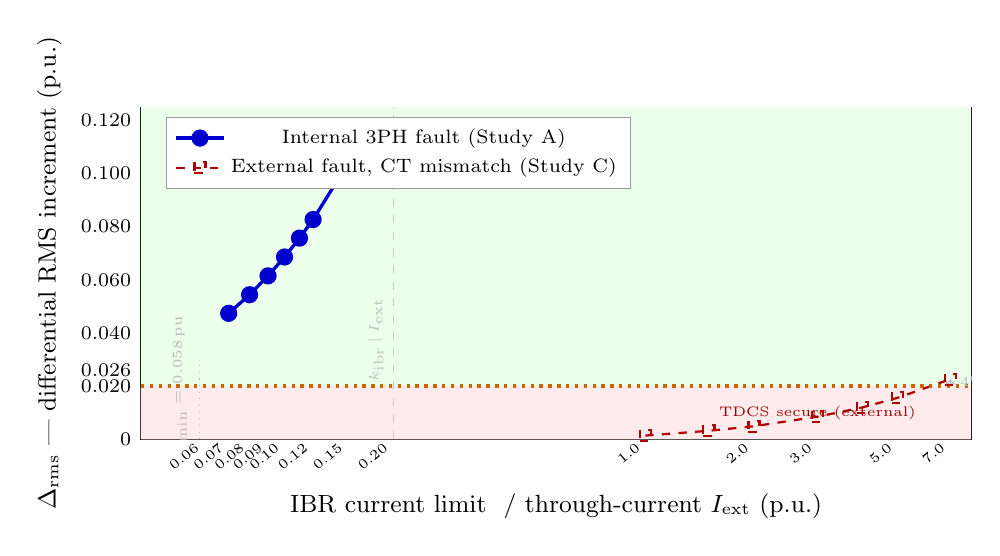
\begin{tikzpicture}
\begin{axis}[
  width=\columnwidth, height=5.8cm,
  xlabel={IBR current limit $\kibr$ / through-current $I_{\rm ext}$ (p.u.)},
  ylabel={$\Delta_{\rm rms}$ — differential RMS increment (p.u.)},
  xmin=0.04, xmax=8.0,
  ymin=0, ymax=0.125,
  xmode=log,
  xtick={0.06,0.07,0.08,0.09,0.10,0.12,0.15,0.20,1.0,2.0,3.0,5.0,7.0},
  xticklabels={0.06,0.07,0.08,0.09,0.10,0.12,0.15,0.20,1.0,2.0,3.0,5.0,7.0},
  xticklabel style={font=\tiny,rotate=40,anchor=east},
  ytick={0,0.020,0.026,0.040,0.060,0.080,0.100,0.120},
  yticklabels={0,0.020,0.026,0.040,0.060,0.080,0.100,0.120},
  yticklabel style={font=\scriptsize},
  grid=both,
  grid style={gray!22,line width=0.3pt},
  tick label style={font=\scriptsize},
  label style={font=\small},
  legend style={at={(0.03,0.97)},anchor=north west,
                font=\scriptsize,fill=white,draw=black!40},
  clip=true]

  % Detect region (above threshold)
  \addplot[fill=green!8,draw=none,forget plot]
    coordinates {(0.04,0.020)(8.0,0.020)(8.0,0.125)(0.04,0.125)} \closedcycle;
  % No-trip region
  \addplot[fill=red!8,draw=none,forget plot]
    coordinates {(0.04,0)(8.0,0)(8.0,0.020)(0.04,0.020)} \closedcycle;

  % Study A: internal fault, delta_I vs k_ibr
  \addplot[blue!80!black,very thick,mark=*,mark size=2.5pt]
    coordinates {
      (0.07, 0.0474)
      (0.08, 0.0544)
      (0.09, 0.0615)
      (0.10, 0.0686)
      (0.11, 0.0757)
      (0.12, 0.0827)
      (0.15, 0.1039)
    };
  \addlegendentry{Internal 3PH fault (Study A)}

  % Study C: external fault, delta_I vs I_ext
  \addplot[red!70!black,thick,dashed,mark=square,mark size=2pt]
    coordinates {
      (1.0, 0.0014)
      (1.5, 0.0032)
      (2.0, 0.0049)
      (3.0, 0.0085)
      (4.0, 0.0120)
      (5.0, 0.0156)
      (7.0, 0.0226)
    };
  \addlegendentry{External fault, CT mismatch (Study C)}

  % Detection threshold
  \draw[orange!80!black,very thick,dotted]
    (axis cs:0.04,0.020) -- (axis cs:8.0,0.020)
    node[right,font=\tiny,orange!80!black]{$\Delta_{\rm thr}=0.020$\,pu};

  % CT mismatch bound annotation at 7 pu
  \draw[<->,gray!55,thin]
    (axis cs:7.0,0.0226) -- (axis cs:7.0,0.0200)
    node[midway,right,font=\tiny,gray!55]{4\% margin};

  % Detection limit annotation
  \draw[gray!55,dotted]
    (axis cs:0.058,0) -- (axis cs:0.058,0.030)
    node[above,font=\tiny,gray!55,rotate=90,pos=0.5]{$k_{\rm ibr,min}=0.058$\,pu};

  % Region labels
  \node[font=\tiny,green!50!black] at (axis cs:0.1,0.105) {TDCS trips (internal)};
  \node[font=\tiny,red!60!black] at (axis cs:3.0,0.010) {TDCS secure (external)};

  % x-axis region separator (between k_ibr and I_ext)
  \draw[gray!40,dashed,thin]
    (axis cs:0.20,0) -- (axis cs:0.20,0.125)
    node[above,font=\tiny,gray!50,rotate=90,pos=0.3]{$k_{\rm ibr}$\,$\vert$\,$I_{\rm ext}$};

\end{axis}
\end{tikzpicture}
